\documentclass[10pt]{article}
\usepackage{graphicx}
\usepackage{amssymb}
\usepackage{epstopdf}
\usepackage{tikz}
\usepackage{enumitem}
\usepackage{multicol,multirow}
\DeclareGraphicsRule{.tif}{png}{.png}{`convert #1 `dirname #1`/`basename #1 .tif`.png}
\renewcommand{\tablename}{Tabla} 
\renewcommand{\figurename}{Figura} 
\newcommand*\circled[1]{\tikz[baseline=(char.base)]{\node[shape=circle,blue,draw,inner sep=1pt] (char) {#1};}}

\usepackage{listings}

\definecolor{mygreen}{rgb}{0,0.6,0}
\definecolor{mygray}{rgb}{0.5,0.5,0.5}
\definecolor{mymauve}{rgb}{0.58,0,0.82}

\lstset{ %
  backgroundcolor=\color{white},   % choose the background color; you must add \usepackage{color} or \usepackage{xcolor}
  basicstyle=\footnotesize,        % the size of the fonts that are used for the code
  breakatwhitespace=false,         % sets if automatic breaks should only happen at whitespace
  breaklines=true,                 % sets automatic line breaking
  captionpos=b,                    % sets the caption-position to bottom
  commentstyle=\color{gray},       % comment style
  deletekeywords={...},            % if you want to delete keywords from the given language
  escapeinside={\%*}{*)},          % if you want to add LaTeX within your code
  extendedchars=true,              % lets you use non-ASCII characters; for 8-bits encodings only, does not work with UTF-8
  frame=none,	                   % adds a frame around the code
  keepspaces=true,                 % keeps spaces in text, useful for keeping indentation of code (possibly needs columns=flexible)
  keywordstyle=\color{blue},       % keyword style
  language=Java,                 % the language of the code
  otherkeywords={else,open},           % if you want to add more keywords to the set
  numbers=left,                    % where to put the line-numbers; possible values are (none, left, right)
  numbersep=20pt,                   % how far the line-numbers are from the code
  numberstyle=\color{mygray}, % the style that is used for the line-numbers
  rulecolor=\color{black},         % if not set, the frame-color may be changed on line-breaks within not-black text (e.g. comments (green here))
  showspaces=false,                % show spaces everywhere adding particular underscores; it overrides 'showstringspaces'
  showstringspaces=false,          % underline spaces within strings only
  showtabs=false,                  % show tabs within strings adding particular underscores
  stepnumber=2,                    % the step between two line-numbers. If it's 1, each line will be numbered
  stringstyle=\color{mymauve},     % string literal style
  tabsize=2,	                   % sets default tabsize to 2 spaces
  title=\lstname                   % show the filename of files included with \lstinputlisting; also try caption instead of title
}
% For a visual definition of these parameters, see
\textwidth = 6.5 in
\textheight = 9 in
\oddsidemargin = 0.0 in
\evensidemargin = 0.0 in
\topmargin = 0.0 in             
\headheight = 0.0 in            
\headsep = 0.0 in
            
\parskip = 0.2in                % vertical space between paragraphs
% Delete the % in the following line if you don't want to have the first line of every paragraph indented
%\parindent = 0.0in

\begin{document}
\begin{center}
    {\Large Prueba Especial, Programaci\'on II} \\
    \emph{\small Prof. Rodrigo Olivares} \\
    \emph{\small Ayud. Juan Carlos Rojas} \\
    \emph{\scriptsize Septiembre 07, 2016}
\end{center}
\vspace*{-35pt}
\begin{center}
    \rule{1\textwidth}{.3pt}
\end{center}
\vspace*{-42pt}
\begin{center}
    \rule{1\textwidth}{2pt}
\end{center}

\vspace*{-15pt}
\textbf{Instrucciones}:
\vspace*{-15pt}

\begin{itemize}
    \item[-] El puntaje m\'aximo de la prueba especial es 100\%, siendo el 60\% el m\'inimo requerido para aprobar.
	\item[-] Responda cada pregunta en el lugar indicado. No se aceptar\'an recorrecciones de pruebas respondidas con l\'apiz grafito.
	\item[-] El tiempo m\'aximo de la evaluaci\'on es de 90 minutos.
    \item[-] La prueba especial es \underline{\textbf{individual}}. Cualquier intento de copia, ser\'a sancionado con nota \textbf{1,0}.
\end{itemize}
\vspace*{-20pt}

\begin{enumerate}

    \item \emph{40pts.} De las siguentes afirmaciones, encierre en un c\'irculo la o las alternativas correctas (\emph{3pts c/u}).    

	{\footnotesize
    
    \begin{multicols}{2}

	\begin{enumerate}[label=(\alph*)]
        \item[i.] La orientaci\'on a objeto es: 
        \item[(a)] Un paradigma de programaci\'on procedural.
        \item[(b)] Un paradigma de programaci\'on estucturado.
        \item[(c)] Una herramienta de programaci\'on.
        \item[(d)] Un lenguaje de programaci\'on.
        \item[\circled{(e)}] Ninguna de las anteriores.
    \end{enumerate}

    \begin{enumerate}[label=(\alph*)]
        \item[ii.] El principio de ocultamiento: 
        \item[(a)] Es una t\'ecnica que protege el estado de una entidad.
        \item[(b)] Es \'util en enfoques procedurales.
        \item[\circled{(c)}] En Java, se logra con los modificadores de acceso.
        \item[(d)] Es encapsular el conocimiento de una entidad.
        \item[(e)] Ninguna de las anteriores.
    \end{enumerate}

    \begin{enumerate}[label=(\alph*)]
        \item[iii.] Una interface:
        \item[(a)] Tiene al menos un m\'etodo implementado.
        \item[\circled{(b)}] Tiene todos sus m\'etodos abstractos.
        \item[\circled{(c)}] Es factible de ser implementada.
        \item[(d)] Es factible de ser extendida.
        \item[(e)] Ninguna de las anteriores.
    \end{enumerate}

    \begin{enumerate}[label=(\alph*)]
        \item[vi.] La herencia m\'ultiple:
        \item[\circled{(a)}] Permite heredar diverso compartimiento.
        \item[\circled{(b)}] Apoya el principio ocultamiento.
        \item[(c)] Apoya el principio de encapsulamiento.
        \item[(d)] En Java se desarrolla implementado clases abstractas.
        \item[\circled{(e)}] En Java se desarrolla implementado interfaces.
    \end{enumerate}

    \begin{enumerate}[label=(\alph*)]
        \item[v.] Un thread: 
		\item[\circled{(a)}] Es un flujo de un proceso en memoria.        
        \item[(b)] Es un proceso que se ejecuta en memoria.
        \item[\circled{(c)}] Puede ser creado como clase en Java.
        \item[(d)] Puede ser instanciado como atributo.
        \item[(e)] Ninguna de las anteriores.
    \end{enumerate}

    \begin{enumerate}[label=(\alph*)]
        \item[vi.] Para una hebra o hilo se debe:
        \item[(a)] Iniciar con el m\'etodo run.
        \item[\circled{(b)}] Iniciar con el m\'etodo start.
        \item[\circled{(c)}] Sobreescribir el m\'etodo run.
        \item[(d)] Sobreescribir el m\'etodo start.
        \item[(e)] Dormir (sleep) la hebra.
    \end{enumerate}

    \begin{enumerate}[label=(\alph*)]
        \item[vii.] En el ciclo de vida de una hebra, el estado: 
        \item[\circled{(a)}] New crea la hebra.
        \item[(b)] Runnable ejecuta siempre la hebra.
        \item[(c)] Blocked se ejecuta, sin importar estados internos.
        \item[(d)] Dead es invocado generalmente por el m\'etodo sleep.
        \item[\circled{(e)}] Yield, verifica el desempe\~no del estado Runnable.
    \end{enumerate}

    \begin{enumerate}[label=(\alph*)]
        \item[viii.] Los bloqueos de recursos compartidos se consiguen:
        \item[(a)] Package, bloqueando los accesos a las clases internas.
        \item[\circled{(b)}] Clase, bloqueando m\'etodos y atributos de la clase.
        \item[(c)] Atributo, declar\'andolos como static.
        \item[\circled{(d)}] Objeto, declarando los m\'etodos como synchronized.
        \item[(e)] Ninguna de las anteriores
    \end{enumerate}

    \begin{enumerate}[label=(\alph*)]
        \item[ix.] Referente a JFrame:
        \item[\circled{(a)}] Habitualmente se usa para crear la ventana principal.
        \item[(b)] getPaneContent() obtiene el panel principal.
        \item[(c)] setAdd() permite agregar componentes al panel.
        \item[\circled{(d)}] setSize() permite dimensionar la ventana.
        \item[(e)] Ninguna de las anteriores
    \end{enumerate}

    \begin{enumerate}[label=(\alph*)]
        \item[x.] Para realizar acciones desde un bot\'on Se requiere:
        \item[(a)] Crear una clase que implemente un ActionEvent.
        \item[\circled{(b)}] Crear una clase que implemente un ActionListener.
        \item[(c)] Re-escribir el m\'etodo actionEvent(ActionPerformed).
        \item[\circled{(d)}] Re-escribir el m\'etodo actionPerformed(ActionEvent).
        \item[\circled{(e)}] Agregar la instancia de la clase oyente, al bot\'on.
    \end{enumerate}

	\end{multicols}
}
    \item \emph{70pts.} Desarrolle una aplicaci\'on en JAVA, con interfaz de usuario que permita mostrar en alg\'un componente de salida, la informaci\'on bancaria de abono y giro de un cliente, simulado por procesos concurrentes. Para ellos se solicita lo siguiente:
    
    \begin{enumerate}[label=(\alph*)]
		\item Construir interfaz de usuario en JAVA que contenga como m\'inimo lo que se muestra en la Figura \ref{fig:graf-user-mt}). Los botones ''Detener'' permiten pausar/dormir el proceso en cuesti\'on, cambiando su etiqueta a ''Procesar''. El bot\'on ''Procesar'' permite despertar/levantar el proceso en cuesti\'on \emph{(20 pts)}.
		\item Construir los procesos concurrentes:
		\begin{enumerate}[label=(\alph*)]
			\item[i.] ProcesoBancoAbono: Permite registrar abonos aleatorios (entre \$1 y \$10.000 CLP) sin l\'imite m\'aximo \emph{(15 pts)}.
			\item[ii.] ProcesoBancoGiro: Permite registrar giros aleatorios (entre \$1 y \$10.000 CLP) sin l\'imite m\'inimo \emph{(15 pts)}.
		\end{enumerate}
		\item Luego de construir los procesos concurrentes, debe desarrollar la clase de recurso compartido \emph{(15 pts)}
		\item Por \'ultimo, desarrolle la clase principal de la aplicaci\'on \emph{(5 pts)}.
	\end{enumerate}

	\begin{figure}[h]
        \begin{center}
            \fbox{\fbox{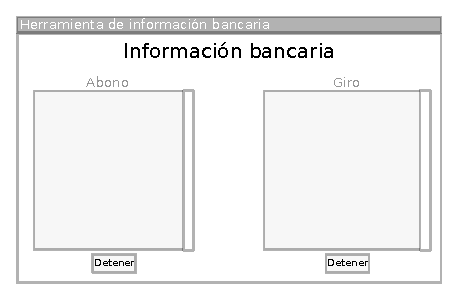
\includegraphics[scale=1]{images/fig-1.pdf}}}
            \caption{Interfaz de usuario}\label{fig:graf-user-mt}
        \end{center}
    \end{figure}
	\end{enumerate}
	\textbf{Interfaz de usuario y m\'etodo principal}

    \lstinputlisting[numbers=none,caption=]{Java/CuentaCorrienteView.java} 	
	
	\textbf{Recurso compartido}
	
	\lstinputlisting[numbers=none,caption=]{Java/CuentaCorriente.java} 	

	\textbf{Proceso Dep\'osito}
	
	\lstinputlisting[numbers=none,caption=]{Java/ThreadCuentaCorrienteDepositar.java} 	
	
	\textbf{Proceso Giro}

    \lstinputlisting[numbers=none,caption=]{Java/ThreadCuentaCorrienteGirar.java} 			

	\textbf{Principal}

    \lstinputlisting[numbers=none,caption=]{Java/Main.java} 			

\end{document} 
